\lab{Solitons}{Solitons}
\label{lab:solitons}
\labdependencies{NumericalIVP,SpectralMethod2}

\objective{Use a pseudospectral method to study solitons, the traveling wave solutions of the Korteweg-de Vries equation.}

The Korteweg-de Vries (KdV) equation is a partial differential equation given by 
\[  \frac{\partial u }{\partial t} + u \frac{\partial u}{\partial x} + \frac{\partial^3 u}{\partial x^3} = 0.
\]
that describes shallow water waves. 

The KdV equation possesses traveling wave solutions called \emph{solitons}.  
These traveling waves have the form 
\[ u(x,t) = 3s \sech^2\left(\frac{\sqrt{s}}{2}(x - st - a)\right),
\]
where $s$ is the speed of the wave. 
Solitons were first studied by John Scott Russell in 1834, in the Union Canal in Scotland. 
When a canal boat suddenly stopped, the water piled up in front of the boat continued moving down the canal in the shape of a pulse.  

Note that there is a soliton solution for each wave speed $s$, and that the amplitude and speed of the soliton determine each other. 
Solitons are nonlinearly stable (bumped waves return to their previous shape), and they maintain their energy as they travel. 
Two interacting solitons will also both maintain their shapes after crossing paths. 

\section*{Numerical solution}
Consider the KdV equation on $[-\pi,\pi]$, together with an appropriate initial condition: 
\begin{align*}
	 &{ }u_t = -\frac{1}{2}\left(u^2 \right)_x - u_{xxx},\\
     &{ }u(x,0) = u_0(x).
\end{align*} 
This form of the equation is slightly more convenient for the approach we will take.
We will suppose the initial condition is equal at the two endpoints; that is, \(u_0(-\pi)=u_0(\pi)\).
This will allow us to use the pseudospectral method to find a numerical approximation for the solution $u(x,t)$.

As a reminder, the pseudospectral method involves writing the solution at each point in time using a set of basis functions, complex exponentials being the most common, and using this representation to convert the PDE into an ODE.
Specifically, we can write any solution \(u(x,t)\) as
\[
u(x,t) = \sum_{k=-\infty}^\infty y_k(t)e^{ikx}.
\]
Recall that \(k\) is known as the wave number.
Note that all time-dependence of the solution is contained in the coefficients.
We can only compute this to some finite precision, so we will choose some \(n\) and truncate the series as
\[
u(x,t) = \sum_{k=-n}^n y_k(t)e^{ikx}.
\]
The objective is to obtain an ordinary differential equation for the coefficients \(y_k(t)\).
We now plug it into the PDE:
\begin{align*}
\frac{\partial}{\partial t}\sum_{k=-n}^n y_k(t)e^{ikx}
&=
-\frac{1}{2} \frac{\partial}{\partial x}\left(
\sum_{k=-n}^n y_k(t)e^{ikx}
\right)^2
-
\frac{\partial^3}{\partial^3 x}\sum_{k=-n}^n y_k(t)e^{ikx}
\\
\sum_{k=-n}^n y_k'(t)e^{ikx}
&=
-\frac{1}{2} \frac{\partial}{\partial x}\left(
\sum_{k=-n}^n y_k(t)e^{ikx}
\right)^2
+
\sum_{k=-n}^n ik^3 y_k(t)e^{ikx}
\end{align*}
For this particular PDE, this leads to an apparent problem: the \(u^2\) term will be difficult and computationally costly to differentiate.
However, we can get around this difficulty using the fast Fourier transform.

Divide \([-\pi, \pi]\) into \(2n+1\) intervals of equal width \(\frac{2\pi}{2n+1}\), and let \(-\pi=x_{-n},x_{-n+1},\ldots,x_n,x_{n+1}=\pi\) be the \(2n+2\) evenly-spaced gridpoints.
For any function \(f\) on that interval with Fourier series \(f(x)=\sum_{k=-\infty}^\infty a_k e^{ikx}\), we can use the discrete Fourier transform on the values \(f(x_{-n}),\ldots,f(x_{n+1})\) at the gridpoints to quickly get the Fourier coefficients \(a_{-n},\ldots, a_n\).
The inverse Fourier transform can be used to get the function values at the grid points from the Fourier coefficients.
Both of these operations are very efficient, having complexity \(O(n\log n)\).
This sets up our strategy.

At each time \(t\), we can use the inverse Fourier transform to compute the values of \(u(x_m,t)\) for \(m=-n,\ldots,n+1\).
Then, we apply the Fourier transform to \(u^2\) to get its Fourier coefficients.
We will denote these as \(w_k\), so
\[
u^2(x,t)=\sum_{k=-n}^n w_k(t) e^{ikx}.
\]
Then, 
\[
\frac{\partial}{\partial x}
u^2(x,t)=\sum_{k=-n}^n ik w_k(t) e^{ikx},
\]
so the KdV equation can be written as
\[
\sum_{k=-n}^n y_k'(t)e^{ikx}
=
\sum_{k=-n}^n \left(
-\frac{1}{2}ikw_k(t)
+
ik^3 y_k(t)
\right)e^{ikx}
\]
Equating terms in the Fourier series yields the ordinary system of differential equations
\[
y_k' = -\frac{1}{2}ikw_k + ik^3 y_k, \quad k=-n,\ldots, n.
\]
We can write this in a vectorized form as
\begin{equation}
\mathbf{y}' = -\frac{1}{2}i\mathbf{k}\odot\mathcal{F}(\mathcal{F}^{-1}(\mathbf{y})^2) + i\mathbf{k}^3 \odot\mathbf{y}
\label{lab:solitons:pseudospectral}
\end{equation}
where \(\mathcal{F}\) denotes the discrete Fourier transform.
In this equation, all of the multiplication and exponentiation is componentwise.

To obtain the initial condition for the \(y_k\), we can simply use the discrete Fourier transform again:
\[
\mathbf{y}(0) = \mathcal{F}(u_0(x_{-n}),\ldots,u_0(x_{n+1}))
\]

To compute the fast Fourier and inverse fast Fourier transforms numerically, we will use the \li{scipy.fft} module, which has functions \li{fft} for the fast Fourier transform and \li{ifft} for the inverse fast Fourier transform.
% it also has \li{rfft} and \li{irfft}, but these are a little funny to work with because the latter treats everything as the positive coefficients because the negative ones are actually redundant; we're just going to not mention them because of that.
These functions use an order for the coefficients that is slightly nonintuitive: the coefficients for \(k\geq 0\) are all listed first, followed by the coefficients for \(k<0\).
The vector of wavenumbers can be created as follows:
\begin{lstlisting}
k = np.concatenate([
        np.arange(0,n+1),
        np.arange(-n-1,0)
])
\end{lstlisting}
We are now prepared to numerically solve the KdV equation.


\begin{comment} %%%% Confusing explanation starts here
\section*{Confusing explanation}
If we use $N$ subintervals in space, we then obtain the spatial step $h = 2\pi/N$ and the grid points $\{x_j\}_{j=1} = \{-\pi,-\pi + h,\ldots,\pi-h\}$.  
Let $\mathcal{F}(u)(t) = \hat{u}(t)$ denote the Fourier transform of $u(x,t)$ (in space), so that 
\[
\mathcal{F}(u) = \hat{u}(k,t), \quad k=-N/2+1, \ldots, N/2.
\]
Similarly we let $\mathcal{F}^{-1}$ represent the discrete inverse Fourier transform.
Recall that $k$ represents the wave numbers in Fourier space; our code defines it by 
\begin{lstlisting}
[BAD CODE THAT USES TABS]
\end{lstlisting}

We now apply the Fourier transform to the KdV equation.
In Fourier space, we obtain 
\begin{align*}
	\mathcal{F}(u)_t &= -\frac{ik}{2}\mathcal{F}(u^2)- (ik)^3\mathcal{F}(u).
\end{align*}
Let $U(t)$ be the vector valued function given by $U(t) = (u(x_j,t))_{j=1}^N$.
Let $\mathcal{F}(U)(t)$ denote the discrete Fourier transform of $u(x,t)$ (in space), so that 
\[
\mathcal{F}(U)(t) = (\mathcal{F}(u)(k,t))_{k=-N/2+1}^{N/2}.
\]
Similarly we let $\mathcal{F}^{-1}$ represent the discrete inverse Fourier transform.
Using the pseudospectral approximation in space leads to the system of ODEs
\begin{align}
	\mathcal{F}(U)_t =  -\frac{i}{2} \vec{k}\mathcal{F}\left( \mathcal{F}^{-1}(\mathcal{F}(U))^2\right) + i\vec{k}^3\mathcal{F}(U)
\end{align}
where $\vec{k}$ is a vector, and multiplication is done element-wise. In terms of $Y = \mathcal{F}(U)$, this simplifies to 
\begin{align}
	Y_t =  -\frac{i}{2} \vec{k}\mathcal{F}\left( \mathcal{F}^{-1}(Y)^2\right) + i\vec{k}^3Y
	\label{lab:solitons:pseudospectral}
\end{align}
and is implemented below.
\begin{lstlisting}
# Defines the left hand side of the ODE y' = G(t,y)
# defined above.
ik3 = 1j*k**3.
def G_unscaled(t,y):
	out = -.5*1j*k*fft(ifft(y,axis=0)**2.,axis=0)  + ik3*y        
	return out
\end{lstlisting}

Equation \eqref{lab:solitons:pseudospectral} is solved below, using a soliton as initial data for the KdV equation. 
Note that the Fourier transform must be applied to the soliton before solving, and that the final numerical solution must be transformed back from Fourier space before plotting. 
\begin{lstlisting}
N = 256
x = (2.*np.pi/N)*np.arange(-N/2,N/2).reshape(N,1)   # Space discretization
s, shift = 25.**2., 2.  							# Initial data is a soliton
y0 = (3.*s*np.cosh(.5*(sqrt(s)*(x+shift)))**(-2.)).reshape(N,) 

# Solves the ODE.
max_t = .0075
dt = .02*N**(-2.)
max_tsteps = int(round(max_t/dt))
y0 = fft(y0,axis=0)
T,Y = RK4(G_unscaled, y0, t0=0, t1=max_t, n=max_tsteps)

# Using the variable stride, we step through the data, 
# applying the inverse fourier transform to obtain u.
# These values will be plotted.
stride = int(np.floor((max_t/25.)/dt))
uvalues, tvalues = np.real(ifft(y0,axis=0)).reshape(N,1), np.array(0.).reshape(1,1)
for n in range(1,max_tsteps+1):
	if np.mod(n,stride) == 0:
		t = n*dt
		u = np.real( ifft(Y[n], axis=0) ).reshape(N,1)
		uvalues = np.concatenate((uvalues,np.nan_to_num(u)),axis=1)
		tvalues = np.concatenate((tvalues,np.array(t).reshape(1,1)),axis=1)

fig = plt.figure()
ax = fig.gca(projection='3d')
ax.view_init(elev=45., azim=150)
tv, xv = np.meshgrid(tvalues,x,indexing='ij')
surf = ax.plot_surface(tv,xv, uvalues.T, rstride=1, cstride=1, cmap=cm.coolwarm,
						linewidth=0, antialiased=False)
tvalues = tvalues[0]; ax.set_xlim(tvalues[0], tvalues[-1])
ax.set_ylim(-pi, pi); ax.invert_yaxis()
ax.set_zlim(0., 4000.)
ax.set_xlabel('T'); ax.set_ylabel('X'); ax.set_zlabel('Z')
plt.show()
\end{lstlisting}

The method we have used requires the use of an algorithm for (ODE) initial value problems, such as the RK4 algorithm.
The RK4 method is implemented below.
\begin{lstlisting}
def initialize_all(y0, t0, t1, n):
	""" An initialization routine for the different ODE solving
	methods in the lab. This initializes Y, T, and h. """
	
	if isinstance(y0, np.ndarray):
		Y = np.empty((n, y0.size),dtype=complex).squeeze()
	else:
		Y = np.empty(n,dtype=complex)
	Y[0] = y0
	T = np.linspace(t0, t1, n)
	h = float(t1 - t0) / (n - 1)
	return Y, T, h

def RK4(f, y0, t0, t1, n):
	""" Use the RK4 method to compute an approximate solution
	to the ODE y' = f(t, y) at n equispaced parameter values from t0 to t
	with initial conditions y(t0) = y0.
	
	'y0' is assumed to be either a constant or a one-dimensional numpy array.
	't0' and 't1' are assumed to be constants.
	'f' is assumed to accept two arguments.
	The first is a constant giving the current value of t.
	The second is a one-dimensional numpy array of the same size as y.
	
	This function returns an array Y of shape (n,) if
	y is a constant or an array of size 1.
	It returns an array of shape (n, y.size) otherwise.
	In either case, Y[i] is the approximate value of y at
	the i'th value of np.linspace(t0, t, n).
	"""
	Y, T, h = initialize_all(y0, t0, t1, n)
	for i in xrange(1, n):
		K1 = f(T[i-1], Y[i-1])
		tplus = (T[i] + T[i-1]) * .5
		K2 = f(tplus, Y[i-1] + .5 * h * K1)
		K3 = f(tplus, Y[i-1] + .5 * h * K2)
		K4 = f(T[i], Y[i-1] + h * K3)
		Y[i] = Y[i-1] + (h / 6.) * (K1 + 2 * K2 + 2 * K3 + K4)
	return T, Y
\end{lstlisting}
\end{comment} % end confusing explanation

\begin{problem}
Write a function that accepts the time value \(t\) (which won't be used here, but will be useful later) the vector \(\mathbf{y}=(y_0,y_1,\ldots,y_n,y_{-n-1},\ldots,y_{-1})\) and the vector \(\mathbf{k}\) of wavenumbers and returns \(\mathbf{y}'\) as given in (\ref{lab:solitons:pseudospectral}).

%\noindent
%Hint: complex numbers are denoted in Python as \li{0.5j}.
\end{problem}

\noindent
To numerically solve this ODE, use the following implementation of the RK4 algorithm:
\begin{lstlisting}
def RK4(f, y0, T, dt, k):
    """
    Solves the ODE y'=f(t, y) using the Runge-Kutta 4 method with initial 
    condition y0 on the time interval [0,T] using a time step of dt.
    The value of k is passed directly into the function f.
    
    Returns:
        t ((n_t,) ndarray) - the time values
        Y ((n_t, 2n+2) ndarray) - the solution values. The solution at the 
                i-th time step can be indexed as Y[i].
    """
    # Set up matrices for the solution
    ts = np.arange(0, T+dt, dt)
    Y = np.empty((len(ts),len(k)), dtype=complex)
    y = y0
    Y[0] = y
    for i in range(1, len(ts)):
        # Use RK4
        t = ts[i]
        K1 = f(t, y, k)
        K2 = f(t + dt/2, y + 0.5*dt*K1, k)
        K3 = f(t + dt/2, y + 0.5*dt*K2, k)
        K4 = f(t + dt, y + dt*K3, k)
        y = y + (dt / 6.) * (K1 + 2*K2 + 2*K3 + K4)
        Y[i] = y
    return ts, Y
\end{lstlisting}

Once we have solved for the coefficients \(\mathbf{y}(t)\), we need to convert them back into function values \(u(x,t)\) in order to visualize the solution.
This is accomplished by using the \li{ifft} function on the coefficient values at each time step.
However, this function is designed to work with complex numbers, and returns a complex-valued array.
Due to numerical error, even though our ODE solution is real-valued, there may be small imaginary components to the result; use \li{np.real} on the result to discard these.

\begin{problem}
Write a function that accepts an initial condition \(u_0\), a final time \li{T}, the timestep \li{dt}, an integer \(n\) for the number of coefficients to use, and another integer \li{skip}.
Numerically solve for the coefficients \(\mathbf{y}(t)\) of a solution to the KdV equation.

Next, convert the Fourier coefficients back into function values at the gridpoints using the inverse Fourier transform.
However, only do this for every \li{skip}-th timestep; we will be using far more timesteps than we want to plot.
Return the gridpoints, the timesteps, and the solution \(u(x,t)\).
\end{problem}

\noindent
Once we have the function values, we can plot them as a surface as follows:
% could always change it to an animation :)
\begin{lstlisting}
fig = plt.figure()
ax = fig.add_subplot(1,1,1, projection='3d')

T, X = np.meshgrid(t, x, indexing='ij')
ax.plot_surface(T, X, u, cmap='coolwarm', rstride=1, cstride=1)
\end{lstlisting}
%This creates a 3-d plot, so the subplot this is done in must be created with \li{projection='3d'}.

\begin{problem}
Numerically solve the KdV equation on $[-\pi,\pi]$ with initial conditions 
\[
u(x,t=0) = 3s\sech^2\left(\frac{\sqrt{s}}{2}(x+a)\right),
\]
where $s = 25^2,$ $a = 2$. Solve on the time domain $[0,0.0075]$, and use \(n=127\).
Compare with Figure \ref{fig:solitons:single}; to get a similar viewpoint, use the following:
\begin{lstlisting}
ax.view_init(elev=45, azim=-45)
ax.set_zlim(0, 4000)
ax.invert_xaxis()
\end{lstlisting} %TODO update the figure
How small of a timestep did you need to use for the numerical integration to be stable?
(Hint: it's smaller than $10^{-5}$.)
If your solution becomes full of NaN values, you are most likely using too large of a timestep.
\label{problem:solitons:single}

\noindent
Hint: \li{numpy} does not have a \li{sech} function; use \li{1/cosh(x)} to compute it instead.
\end{problem}

\begin{figure}[H]
\centering
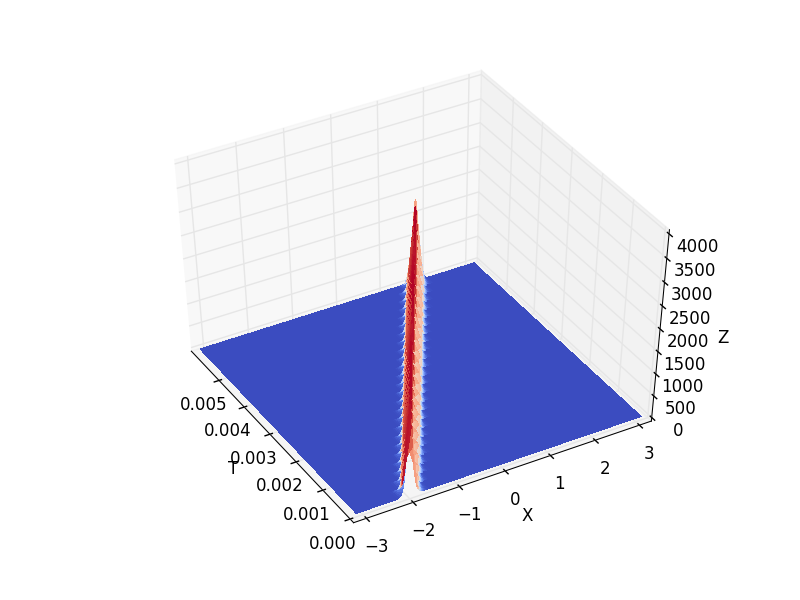
\includegraphics[width=\textwidth]{figures/soliton.png}
\caption{The solution to Problem \ref{problem:solitons:single}.}
\label{fig:solitons:single}
\end{figure}

\begin{problem}
Numerically solve the KdV equation on $[-\pi,\pi]$.
This time we define the initial condition 
to be the superposition of two solitons:
\[
u(x,t=0) = 3s_1\sech^2\left(\frac{\sqrt{s_1}}{2}(x+a_1)\right) + 3s_2\sech^2\left(\frac{\sqrt{s_2}}{2}(x+a_2)\right),
\]
where $s_1 = 25^2,$ $a_1 = 2$, and $s_2 = 16^2,$ $a_2 = 1$.\footnote{This problem is from \textit{Spectral Methods in MATLAB}, by Trefethen.}
Solve on the time domain $[0,0.0075]$.
The solution is shown in Figure \ref{fig:solitons:interacting}.
\label{problem:solitons:interacting}
\end{problem}

\begin{figure}[H]
\centering
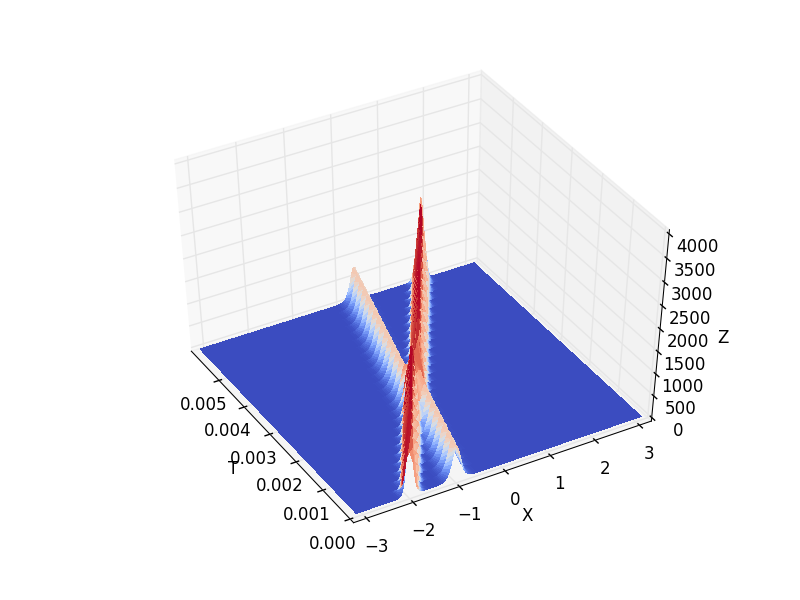
\includegraphics[width=\textwidth]{figures/interacting_solitons.png}
\caption{The solution to Problem \ref{problem:solitons:interacting}.}
\label{fig:solitons:interacting}
\end{figure}

\begin{problem}
Consider again equation \eqref{lab:solitons:pseudospectral}.
The linear term in this equation is $i\mathbf{k}^3\mathbf{y}$.
This term contributes much of the exponential growth in the ODE, and contributes to how short the time step must be to ensure numerical stability.
Make the substitution $z_k(t) = e^{-ik^3t}y_k(t)$ and find a similar ODE for $\mathbf{z}$.
This essentially allows the exponential growth to be scaled out (it's solved for analytically, replacing it with rotation in the complex plane).
Use the resulting equation to solve the previous problem.
How much larger of a timestep can you use while this method remains stable?
\end{problem}